% 四大数学奖交叉汇总名录 · Four Major Mathematics Awards — Cross-Reference
% Fields Medal · Wolf Prize · Abel Prize · Chern Medal
% 重点：标注同时获得多个奖项的数学家（交叉获奖），并附中文名字
% Compile with: xelatex math_awards_allinone.tex   (或 make)
% Data: Wikipedia, IMU, Wolf Foundation, Norwegian Academy of Science and Letters

\documentclass[a4paper,10pt]{article}

% ---- Fonts & Language ----
\usepackage{fontspec}
\usepackage{xeCJK}
\setCJKmainfont{PingFang SC}[BoldFont=PingFang SC Semibold]
\setCJKsansfont{PingFang SC}
\setmainfont{Times New Roman}[BoldFont=Times New Roman Bold]
\setsansfont{Helvetica Neue}

% ---- Layout ----
\usepackage[margin=1.2cm,top=1.8cm,bottom=1.8cm,landscape]{geometry}
\usepackage{longtable}
\usepackage{booktabs}
\usepackage{array}
\usepackage{xcolor}
\usepackage{colortbl}
\usepackage{fancyhdr}
\usepackage{tikz}
\usepackage{hyperref}
\usepackage{amssymb}

% ---- Colors ----
\definecolor{headerblue}{RGB}{41,65,122}
\definecolor{headerbg}{RGB}{220,230,245}
\definecolor{rowalt}{RGB}{245,248,252}
\definecolor{yearcolor}{RGB}{180,50,50}
\definecolor{fieldcolor}{RGB}{30,100,60}
\definecolor{mutedgray}{RGB}{100,100,100}
\definecolor{congressbg}{RGB}{255,245,225}
% ---- Per-award brand colors (for badges) ----
\definecolor{fieldsclr}{RGB}{41,65,122}   % Fields  — 深蓝
\definecolor{wolfclr}{RGB}{180,120,0}     % Wolf    — 金棕
\definecolor{abelclr}{RGB}{150,40,90}     % Abel    — 紫红
\definecolor{chernclr}{RGB}{15,110,92}    % Chern   — 翡翠绿
\definecolor{triplebg}{RGB}{255,236,236}  % 三奖高亮
\definecolor{doublebg}{RGB}{240,245,255}  % 双奖高亮

\hypersetup{colorlinks=true, linkcolor=headerblue, urlcolor=fieldcolor}

% ---- Page Style ----
\pagestyle{fancy}
\fancyhf{}
\fancyhead[L]{\small\sffamily\color{headerblue} 数学「大满贯」俱乐部 · Fields · Wolf · Abel · Chern}
\fancyhead[R]{\small\sffamily\color{headerblue} 1936–2026 · 交叉获奖标注}
\fancyfoot[C]{\small\sffamily\thepage}
\renewcommand{\headrulewidth}{0.4pt}

% ---- Award badges ----
% 每个奖一个彩色徽标，右上角标注；用于名字后缀
\newcommand{\Fbadge}{\textsuperscript{\normalfont\scriptsize\sffamily\color{fieldsclr}$\blacklozenge$F}}
\newcommand{\Wbadge}{\textsuperscript{\normalfont\scriptsize\sffamily\color{wolfclr}$\bigstar$W}}
\newcommand{\Abadge}{\textsuperscript{\normalfont\scriptsize\sffamily\color{abelclr}$\blacktriangle$A}}
\newcommand{\Cbadge}{\textsuperscript{\normalfont\scriptsize\sffamily\color{chernclr}$\blacksquare$C}}

% 交叉名录行：#1=英文名 #2=中文名 #3=四奖徽标串 #4=各奖年份 #5=国籍 #6=领域
\newcommand{\crossrow}[6]{%
  {\bfseries #1}\,{\small\color{mutedgray}#2} #3 & {\small #4} & {\small #5} & {\small\color{fieldcolor}#6} \\[2pt]
}

% 单奖名录（Fields 主表沿用）：#1=Name #2=Award(age) #3=生卒 #4=国籍 #5=机构 #6=领域
\newcommand{\congressheader}[2]{%
  \rowcolor{congressbg}
  \multicolumn{6}{l}{%
    \raisebox{0pt}[1.2em][0.4em]{%
      \bfseries\sffamily\color{yearcolor} \large #1 \normalsize
      \color{mutedgray}\enspace #2%
    }%
  } \\
  \midrule
}
\newcommand{\laureaterow}[6]{%
  {\bfseries #1} & {\color{yearcolor}#2} & {#3} & {#4} & {\small #5} & {\small\color{fieldcolor}#6} \\[2pt]
}

% ---- Document ----
\begin{document}

\begin{center}
  \vspace*{0.2em}
  {\Huge\bfseries\sffamily\color{headerblue} 数学「大满贯」俱乐部 —— 四大奖项交叉名录}\\[6pt]
  {\Large\sffamily\color{headerblue} Fields · Wolf · Abel · Chern}\\[6pt]
  {\normalsize\color{mutedgray} 双料冠军 · 三冠传奇 · 全满贯得主 · 1936–2026}\\[3pt]
  {\small\color{mutedgray} Data: Wikipedia · IMU · Wolf Foundation · Norwegian Academy of Science and Letters}
\end{center}

\vspace{0.6em}

% ===== 图例 =====
\begin{center}
\colorbox{headerbg}{\parbox{0.92\textwidth}{\centering\small
    \textbf{徽标图例}：\quad
    {\color{fieldsclr}$\blacklozenge$\,F} 菲尔兹奖 Fields（$\le$40 岁，四年一届，IMU）\quad
    {\color{wolfclr}$\bigstar$\,W} 沃尔夫奖 Wolf（无年龄限制，每年，以色列）\\[3pt]
    {\color{abelclr}$\blacktriangle$\,A} 阿贝尔奖 Abel（无年龄限制，每年，挪威）\quad
    {\color{chernclr}$\blacksquare$\,C} 陈省身奖章 Chern（无年龄限制，四年一届，IMU）\\[4pt]
    {\color{mutedgray}\itshape 名字后徽标越多，代表其横跨的顶级奖项越多；下方「交叉获奖」章节按获奖数量高亮排列。}}}
\end{center}

\vspace{0.8em}

% ===== Medal images =====
\begin{center}
  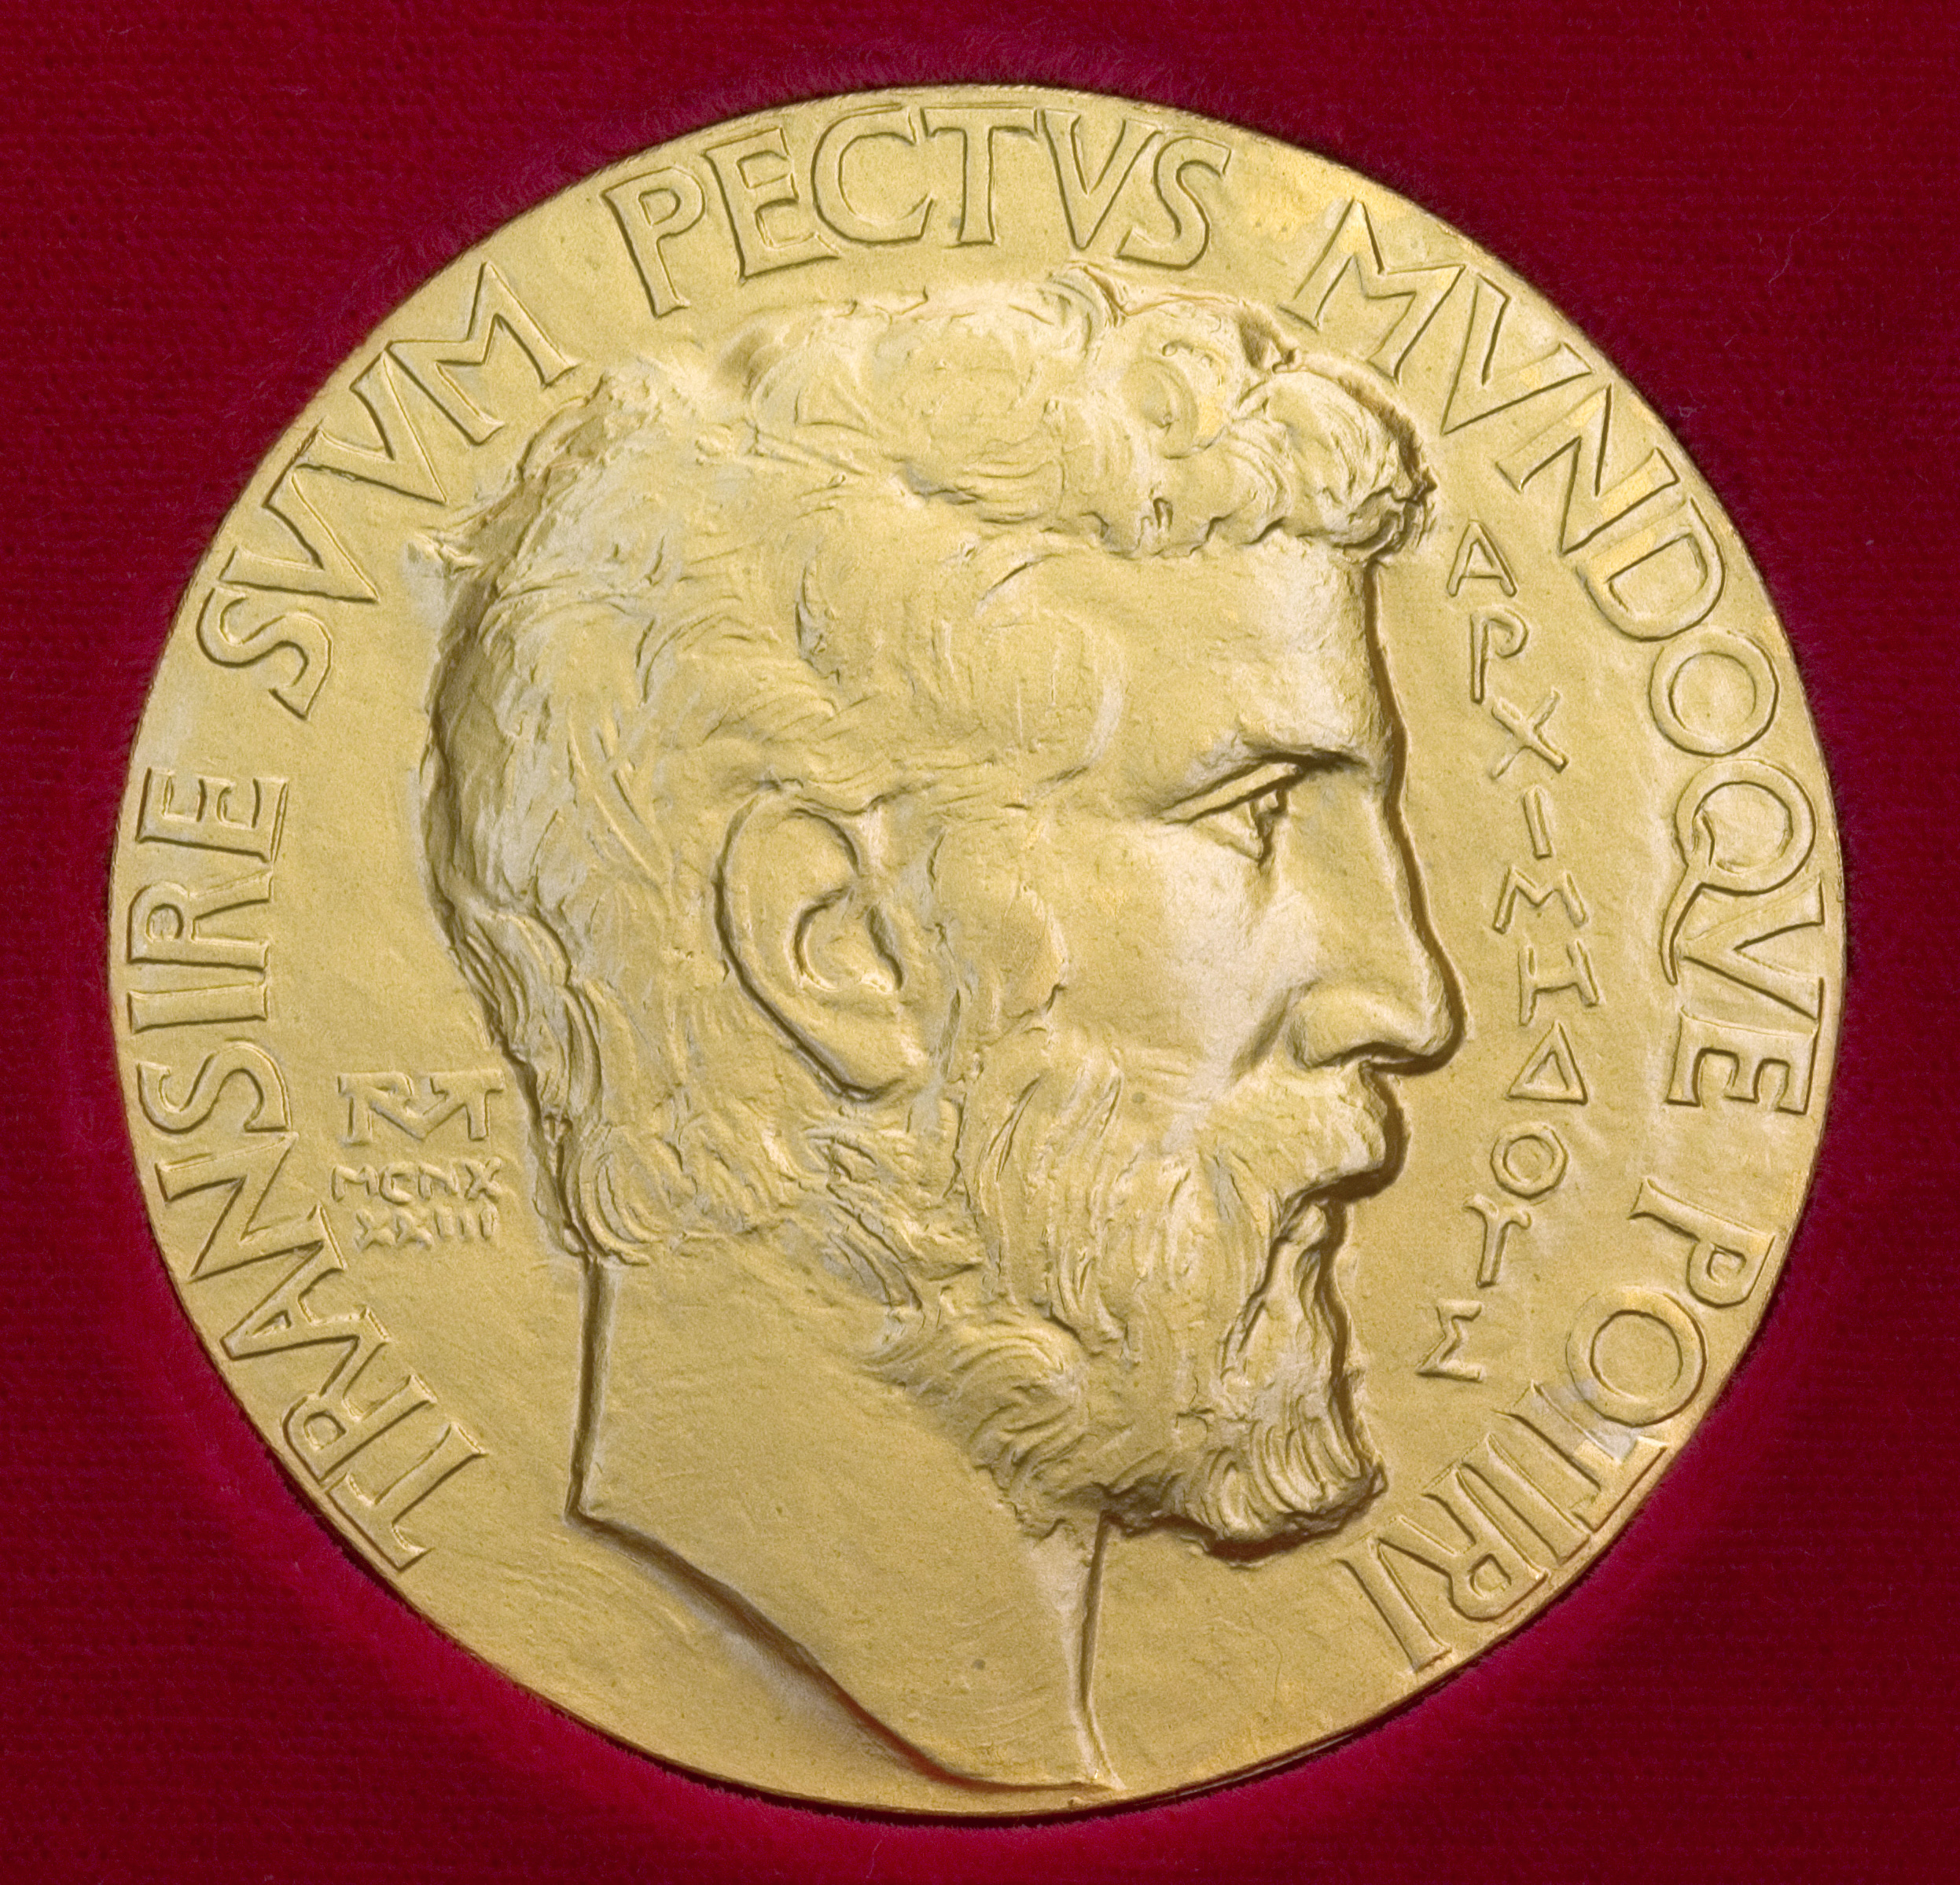
\includegraphics[height=3.5cm]{cover/FieldsMedalFront_hires.jpg}\hspace{2cm}
  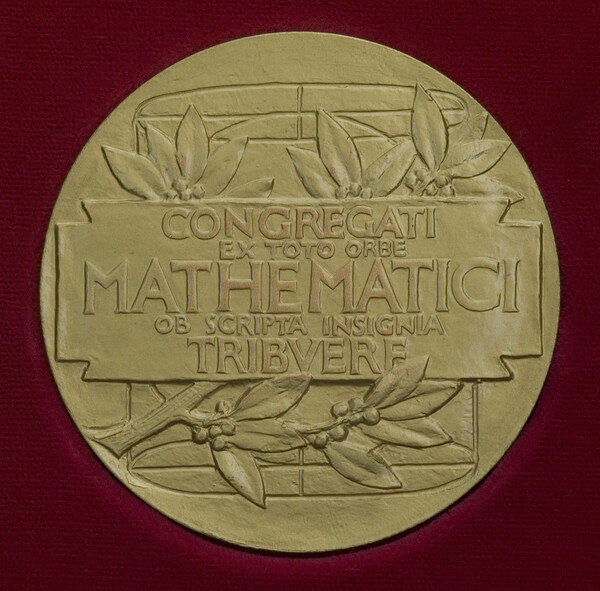
\includegraphics[height=3.5cm]{cover/FieldsMedalBack_600px.jpg}
\end{center}

\vspace{0.6em}

% ============================================================
% PART I — 交叉获奖名录（多奖得主）
% ============================================================
\begin{center}
  {\LARGE\bfseries\sffamily\color{headerblue} 第一部分 · 交叉获奖名录}\\[3pt]
  {\small\color{mutedgray} 同时获得两个及以上顶级数学奖的数学家 · 共 33 人}
\end{center}

\vspace{0.5em}

\begin{longtable}{
  >{\raggedright}m{6.2cm}
  >{\raggedright}m{5.2cm}
  >{\raggedright}m{2.6cm}
  >{\raggedright\arraybackslash}m{9.0cm}
}
\toprule
\rowcolor{headerbg}
\textbf{\sffamily 姓名 Name（徽标）} &
\textbf{\sffamily 获奖年份 Awards} &
\textbf{\sffamily 国籍} &
\textbf{\sffamily 研究领域 Field} \\
\midrule
\endfirsthead
\toprule
\rowcolor{headerbg}
\textbf{\sffamily 姓名 Name（徽标）} &
\textbf{\sffamily 获奖年份 Awards} &
\textbf{\sffamily 国籍} &
\textbf{\sffamily 研究领域 Field} \\
\midrule
\endhead
\midrule
\multicolumn{4}{r}{\small\itshape 续下页 \ldots} \\
\endfoot
\bottomrule
\endlastfoot

%% ===== 三奖：Fields + Wolf + Abel（5 人）=====
\rowcolor{triplebg}
\multicolumn{4}{l}{\raisebox{0pt}[1.2em][0.4em]{\bfseries\sffamily\color{yearcolor}\large ★★★ 三奖得主 · Fields + Wolf + Abel \normalsize \color{mutedgray}\enspace 数学界的「大满贯」（5 人）}} \\
\midrule

\crossrow{Jean-Pierre Serre}{让-皮埃尔·塞尔}{\Fbadge\Wbadge\Abadge}{F 1954 · W 2000 · A 2003}{法国}{代数拓扑、代数几何、数论；史上最年轻菲尔兹奖（27 岁），首届阿贝尔奖}
\crossrow{John Milnor}{约翰·米尔诺}{\Fbadge\Wbadge\Abadge}{F 1962 · W 1989 · A 2011}{美国}{微分拓扑、异国球面、K 理论、动力系统}
\crossrow{John G. Thompson}{约翰·汤普森}{\Fbadge\Wbadge\Abadge}{F 1970 · W 1992 · A 2008}{美国}{有限群论、奇阶定理、有限单群分类}
\crossrow{Pierre Deligne}{皮埃尔·德利涅}{\Fbadge\Wbadge\Abadge}{F 1978 · W 2008 · A 2013}{比利时}{代数几何、Weil 猜想、Hodge 理论}
\crossrow{Grigory Margulis}{格里戈里·马尔古利斯}{\Fbadge\Wbadge\Abadge}{F 1978 · W 2005 · A 2020}{苏联/美国}{Lie 群格、刚性理论、遍历理论}
\midrule

%% ===== 双奖：Fields + Wolf（11 人）=====
\rowcolor{doublebg}
\multicolumn{4}{l}{\raisebox{0pt}[1.2em][0.4em]{\bfseries\sffamily\color{fieldsclr}\large ★★ 双奖 · Fields + Wolf \normalsize \color{mutedgray}\enspace 早年突破 + 终身成就（11 人）}} \\
\midrule

\crossrow{Lars Ahlfors}{拉尔斯·阿尔福斯}{\Fbadge\Wbadge}{F 1936 · W 1981}{芬兰/美国}{复分析、黎曼曲面、拟共形映射；首位菲尔兹+沃尔夫双奖者}
\crossrow{Atle Selberg}{阿特勒·塞尔伯格}{\Fbadge\Wbadge}{F 1950 · W 1986}{挪威/美国}{解析数论、筛法、Selberg 迹公式}
\crossrow{Kunihiko Kodaira}{小平邦彦}{\Fbadge\Wbadge}{F 1954 · W 1984}{日本}{复流形、代数曲面分类、Hodge 理论}
\crossrow{Lars Hörmander}{拉尔斯·赫尔曼德}{\Fbadge\Wbadge}{F 1962 · W 1988}{瑞典}{线性偏微分算子、微局部分析}
\crossrow{Stephen Smale}{斯蒂芬·斯梅尔}{\Fbadge\Wbadge}{F 1966 · W 2006}{美国}{微分拓扑、高维庞加莱猜想、动力系统}
\crossrow{Sergei Novikov}{谢尔盖·诺维科夫}{\Fbadge\Wbadge}{F 1970 · W 2005}{苏联/俄罗斯}{代数拓扑、Pontryagin 类、孤立子理论}
\crossrow{David Mumford}{大卫·芒福德}{\Fbadge\Wbadge}{F 1974 · W 2008}{美国}{代数几何、模空间、几何不变量理论}
\crossrow{Charles Fefferman}{查尔斯·费弗曼}{\Fbadge\Wbadge}{F 1978 · W 2017}{美国}{多复变、调和分析、PDE}
\crossrow{Shing-Tung Yau}{丘成桐}{\Fbadge\Wbadge}{F 1982 · W 2010}{中国/美国}{微分几何、Calabi 猜想、几何分析；首位华人菲尔兹+沃尔夫双奖}
\crossrow{Simon Donaldson}{西蒙·唐纳森}{\Fbadge\Wbadge}{F 1986 · W 2020}{英国}{四维流形、规范理论、Donaldson 不变量}
\crossrow{Vladimir Drinfeld}{弗拉基米尔·德林费尔德}{\Fbadge\Wbadge}{F 1990 · W 2018}{乌克兰/美国}{Langlands 纲领、量子群、几何 Langlands}
\midrule

%% ===== 双奖：Wolf + Abel（12 人）=====
\rowcolor{doublebg}
\multicolumn{4}{l}{\raisebox{0pt}[1.2em][0.4em]{\bfseries\sffamily\color{wolfclr}\large ★★ 双奖 · Wolf + Abel \normalsize \color{mutedgray}\enspace 两大终身成就奖（12 人）}} \\
\midrule

\crossrow{Peter Lax}{彼得·拉克斯}{\Wbadge\Abadge}{W 1987 · A 2005}{匈牙利/美国}{偏微分方程、泛函分析、Lax 对}
\crossrow{Lennart Carleson}{伦纳特·卡尔松}{\Wbadge\Abadge}{W 1992 · A 2006}{瑞典}{调和分析、Carleson 定理、动力系统}
\crossrow{Jacques Tits}{雅克·蒂茨}{\Wbadge\Abadge}{W 1993 · A 2008}{比利时/法国}{群论、建筑理论、Tits 系}
\crossrow{Mikhail Gromov}{米哈伊尔·格罗莫夫}{\Wbadge\Abadge}{W 1993 · A 2009}{俄罗斯/法国}{黎曼几何、辛几何、几何群论}
\crossrow{Andrew Wiles}{安德鲁·怀尔斯}{\Wbadge\Abadge}{W 1995 · A 2016}{英国}{证明费马大定理；曾获 IMU 特别银质纪念奖}
\crossrow{Robert Langlands}{罗伯特·朗兰兹}{\Wbadge\Abadge}{W 1995 · A 2018}{加拿大/美国}{Langlands 纲领，连接数论、表示论与调和分析}
\crossrow{Yakov Sinai}{雅科夫·西奈}{\Wbadge\Abadge}{W 1996 · A 2014}{俄罗斯/美国}{动力系统、遍历理论、统计力学数学基础}
\crossrow{László Lovász}{拉斯洛·洛瓦兹}{\Wbadge\Abadge}{W 1999 · A 2021}{匈牙利}{组合数学、图论、LLL 算法}
\crossrow{John Tate}{约翰·泰特}{\Wbadge\Abadge}{W 2002 · A 2010}{美国}{数论、Tate 论题、Tate-Shafarevich 群}
\crossrow{Hillel Furstenberg}{希勒尔·富斯滕伯格}{\Wbadge\Abadge}{W 2006 · A 2020}{以色列/美国}{遍历理论、概率、组合数论}
\crossrow{Dennis Sullivan}{丹尼斯·苏利文}{\Wbadge\Abadge}{W 2010 · A 2022}{美国}{拓扑、有理同伦论、复动力系统}
\crossrow{Luis Caffarelli}{路易斯·卡法雷利}{\Wbadge\Abadge}{W 2012 · A 2023}{阿根廷/美国}{非线性 PDE、自由边界问题、最优传输}
\midrule

%% ===== 双奖：Fields + Abel（2 人）=====
\rowcolor{doublebg}
\multicolumn{4}{l}{\raisebox{0pt}[1.2em][0.4em]{\bfseries\sffamily\color{abelclr}\large ★★ 双奖 · Fields + Abel（2 人）}} \\
\midrule

\crossrow{Michael Atiyah}{迈克尔·阿蒂亚}{\Fbadge\Abadge}{F 1966 · A 2004}{英国}{K 理论、Atiyah–Singer 指标定理}
\crossrow{Gerd Faltings}{格尔德·法尔廷斯}{\Fbadge\Abadge}{F 1986 · A 2026}{德国}{算术代数几何、Mordell 猜想}
\midrule

%% ===== 双奖：Wolf + Chern（1 人）=====
\rowcolor{doublebg}
\multicolumn{4}{l}{\raisebox{0pt}[1.2em][0.4em]{\bfseries\sffamily\color{chernclr}\large ★★ 双奖 · Wolf + Chern（1 人）}} \\
\midrule

\crossrow{Phillip Griffiths}{菲利普·格里菲斯}{\Wbadge\Cbadge}{W 2008 · C 2014}{美国}{代数几何、Hodge 理论、Griffiths 横截性}
\midrule

%% ===== 双奖：Abel + Chern（2 人）=====
\rowcolor{doublebg}
\multicolumn{4}{l}{\raisebox{0pt}[1.2em][0.4em]{\bfseries\sffamily\color{chernclr}\large ★★ 双奖 · Abel + Chern（2 人）}} \\
\midrule

\crossrow{Louis Nirenberg}{路易·尼伦伯格}{\Cbadge\Abadge}{C 2010 · A 2015}{加拿大/美国}{非线性椭圆型偏微分方程；首届陈省身奖章}
\crossrow{Masaki Kashiwara}{柏原正树}{\Cbadge\Abadge}{C 2018 · A 2025}{日本}{代数分析、表示论、D-模理论}

\end{longtable}

\vspace{0.5em}
\begin{center}
\colorbox{triplebg}{\parbox{0.9\textwidth}{\centering\small\color{mutedgray}
    \textbf{交叉获奖统计}：共 33 位数学家横跨多奖 ---
    三奖（Fields+Wolf+Abel）\textbf{5} 人 ·
    Fields+Wolf \textbf{11} 人 ·
    Wolf+Abel \textbf{12} 人 ·
    Fields+Abel \textbf{2} 人 ·
    Wolf+Chern \textbf{1} 人 ·
    Abel+Chern \textbf{2} 人。\\[3pt]
    尚无人同时获得全部四奖；陈省身奖章（2010 年起、仅 5 位得主）尚未与 Fields 交叉。}}
\end{center}

\newpage

% ============================================================
% PART II — 四大奖完整名录
% ============================================================
\begin{center}
  {\LARGE\bfseries\sffamily\color{headerblue} 第二部分 · 四大奖完整名录}\\[3pt]
  {\small\color{mutedgray} 名字后徽标标注该得主还获得的其他顶级奖项}
\end{center}

\vspace{0.6em}

% ---------- 陈省身奖章 ----------
\begin{center}{\Large\bfseries\sffamily\color{chernclr} $\blacksquare$ 陈省身奖章 Chern Medal}\quad{\small\color{mutedgray} 2010– · 四年一届 · IMU · 共 5 位}\end{center}
\vspace{0.3em}
\begin{longtable}{
  >{\raggedright}m{1.4cm}
  >{\raggedright}m{6.5cm}
  >{\raggedright}m{5.5cm}
  >{\raggedright\arraybackslash}m{9.0cm}
}
\toprule
\rowcolor{headerbg}
\textbf{\sffamily 年份} & \textbf{\sffamily 姓名 Name} & \textbf{\sffamily 机构} & \textbf{\sffamily 关键词} \\
\midrule
\endhead
{\color{yearcolor}2010} & {\bfseries Louis Nirenberg}\Abadge\,{\small\color{mutedgray}路易·尼伦伯格} & 纽约大学库朗研究所 & {\small\color{fieldcolor}非线性椭圆型偏微分方程；亦获 2015 阿贝尔奖} \\[2pt]
{\color{yearcolor}2014} & {\bfseries Phillip Griffiths}\Wbadge\,{\small\color{mutedgray}菲利普·格里菲斯} & 普林斯顿高等研究院 & {\small\color{fieldcolor}复几何、Hodge 理论；亦获 2008 沃尔夫奖} \\[2pt]
{\color{yearcolor}2018} & {\bfseries Masaki Kashiwara}\Abadge\,{\small\color{mutedgray}柏原正树} & 京都大学数理解析研究所 & {\small\color{fieldcolor}代数分析、表示论、D-模；亦获 2025 阿贝尔奖} \\[2pt]
{\color{yearcolor}2022} & {\bfseries Barry Mazur}\,{\small\color{mutedgray}巴里·梅休} & 哈佛大学 & {\small\color{fieldcolor}拓扑、算术几何、数论} \\[2pt]
{\color{yearcolor}2026} & {\bfseries Graeme Segal}\,{\small\color{mutedgray}格雷姆·西格尔} & 牛津大学 & {\small\color{fieldcolor}拓扑、数学物理、表示论、范畴论} \\[2pt]
\bottomrule
\end{longtable}

\vspace{0.6em}

% ---------- 阿贝尔奖 ----------
\begin{center}{\Large\bfseries\sffamily\color{abelclr} $\blacktriangle$ 阿贝尔奖 Abel Prize}\quad{\small\color{mutedgray} 2003– · 每年 · 挪威科学与文学院 · 共 29 位}\end{center}
\vspace{0.3em}
\begin{longtable}{
  >{\raggedright}m{1.4cm}
  >{\raggedright}m{7.0cm}
  >{\raggedright}m{4.5cm}
  >{\raggedright\arraybackslash}m{9.5cm}
}
\toprule
\rowcolor{headerbg}
\textbf{\sffamily 年份} & \textbf{\sffamily 姓名 Name} & \textbf{\sffamily 国籍} & \textbf{\sffamily 获奖领域 / 关键词} \\
\midrule
\endfirsthead
\toprule
\rowcolor{headerbg}
\textbf{\sffamily 年份} & \textbf{\sffamily 姓名 Name} & \textbf{\sffamily 国籍} & \textbf{\sffamily 获奖领域 / 关键词} \\
\midrule
\endhead
\midrule
\multicolumn{4}{r}{\small\itshape 续下页 \ldots} \\
\endfoot
\bottomrule
\endlastfoot
{\color{yearcolor}2003} & {\bfseries Jean-Pierre Serre}\Fbadge\Wbadge\,{\small\color{mutedgray}让-皮埃尔·塞尔} & 法国 & {\small\color{fieldcolor}拓扑、代数几何、数论；亦获 F1954 / W2000} \\[2pt]
{\color{yearcolor}2004} & {\bfseries Michael Atiyah}\Fbadge\,{\small\color{mutedgray}迈克尔·阿蒂亚} & 英国 & {\small\color{fieldcolor}Atiyah–Singer 指标定理；亦获 F1966} \\[2pt]
{\color{yearcolor}2004} & {\bfseries Isadore Singer}\,{\small\color{mutedgray}伊萨多·辛格} & 美国 & {\small\color{fieldcolor}Atiyah–Singer 指标定理} \\[2pt]
{\color{yearcolor}2005} & {\bfseries Peter Lax}\Wbadge\,{\small\color{mutedgray}彼得·拉克斯} & 匈牙利/美国 & {\small\color{fieldcolor}偏微分方程；亦获 W1987} \\[2pt]
{\color{yearcolor}2006} & {\bfseries Lennart Carleson}\Wbadge\,{\small\color{mutedgray}伦纳特·卡尔松} & 瑞典 & {\small\color{fieldcolor}调和分析、动力系统；亦获 W1992} \\[2pt]
{\color{yearcolor}2007} & {\bfseries S. R. Srinivasa Varadhan}\,{\small\color{mutedgray}斯里尼瓦瑟·瓦拉德汉} & 印度/美国 & {\small\color{fieldcolor}概率论、大偏差理论} \\[2pt]
{\color{yearcolor}2008} & {\bfseries John G. Thompson}\Fbadge\Wbadge\,{\small\color{mutedgray}约翰·汤普森} & 美国 & {\small\color{fieldcolor}群论；亦获 F1970 / W1992} \\[2pt]
{\color{yearcolor}2008} & {\bfseries Jacques Tits}\Wbadge\,{\small\color{mutedgray}雅克·蒂茨} & 比利时/法国 & {\small\color{fieldcolor}群论、建筑理论；亦获 W1993} \\[2pt]
{\color{yearcolor}2009} & {\bfseries Mikhail Gromov}\Wbadge\,{\small\color{mutedgray}米哈伊尔·格罗莫夫} & 俄罗斯/法国 & {\small\color{fieldcolor}几何；亦获 W1993} \\[2pt]
{\color{yearcolor}2010} & {\bfseries John Tate}\Wbadge\,{\small\color{mutedgray}约翰·泰特} & 美国 & {\small\color{fieldcolor}数论；亦获 W2002} \\[2pt]
{\color{yearcolor}2011} & {\bfseries John Milnor}\Fbadge\Wbadge\,{\small\color{mutedgray}约翰·米尔诺} & 美国 & {\small\color{fieldcolor}拓扑、几何、代数；亦获 F1962 / W1989} \\[2pt]
{\color{yearcolor}2012} & {\bfseries Endre Szemerédi}\,{\small\color{mutedgray}安德烈·塞迈雷迪} & 匈牙利/美国 & {\small\color{fieldcolor}离散数学、理论计算机科学} \\[2pt]
{\color{yearcolor}2013} & {\bfseries Pierre Deligne}\Fbadge\Wbadge\,{\small\color{mutedgray}皮埃尔·德利涅} & 比利时 & {\small\color{fieldcolor}代数几何；亦获 F1978 / W2008} \\[2pt]
{\color{yearcolor}2014} & {\bfseries Yakov Sinai}\Wbadge\,{\small\color{mutedgray}雅科夫·西奈} & 俄罗斯/美国 & {\small\color{fieldcolor}动力系统、遍历论、数学物理；亦获 W1996} \\[2pt]
{\color{yearcolor}2015} & {\bfseries John F. Nash Jr.}\,{\small\color{mutedgray}约翰·纳什} & 美国 & {\small\color{fieldcolor}非线性偏微分方程} \\[2pt]
{\color{yearcolor}2015} & {\bfseries Louis Nirenberg}\Cbadge\,{\small\color{mutedgray}路易·尼伦伯格} & 加拿大/美国 & {\small\color{fieldcolor}非线性偏微分方程；亦获 C2010} \\[2pt]
{\color{yearcolor}2016} & {\bfseries Andrew Wiles}\Wbadge\,{\small\color{mutedgray}安德鲁·怀尔斯} & 英国 & {\small\color{fieldcolor}数论、费马大定理；亦获 W1995} \\[2pt]
{\color{yearcolor}2017} & {\bfseries Yves Meyer}\,{\small\color{mutedgray}伊夫·梅耶} & 法国 & {\small\color{fieldcolor}小波分析} \\[2pt]
{\color{yearcolor}2018} & {\bfseries Robert Langlands}\Wbadge\,{\small\color{mutedgray}罗伯特·朗兰兹} & 加拿大/美国 & {\small\color{fieldcolor}Langlands 纲领；亦获 W1995} \\[2pt]
{\color{yearcolor}2019} & {\bfseries Karen Uhlenbeck}\,{\small\color{mutedgray}凯伦·乌伦贝克} & 美国 & {\small\color{fieldcolor}几何分析、规范场论；首位女性阿贝尔奖} \\[2pt]
{\color{yearcolor}2020} & {\bfseries Hillel Furstenberg}\Wbadge\,{\small\color{mutedgray}希勒尔·富斯滕伯格} & 以色列/美国 & {\small\color{fieldcolor}遍历论；亦获 W2006} \\[2pt]
{\color{yearcolor}2020} & {\bfseries Gregory Margulis}\Fbadge\Wbadge\,{\small\color{mutedgray}格里戈里·马尔古利斯} & 俄罗斯/美国 & {\small\color{fieldcolor}群论、遍历论；亦获 F1978 / W2005} \\[2pt]
{\color{yearcolor}2021} & {\bfseries László Lovász}\Wbadge\,{\small\color{mutedgray}拉斯洛·洛瓦兹} & 匈牙利 & {\small\color{fieldcolor}理论计算机科学、离散数学；亦获 W1999} \\[2pt]
{\color{yearcolor}2021} & {\bfseries Avi Wigderson}\,{\small\color{mutedgray}阿维·维格森} & 以色列/美国 & {\small\color{fieldcolor}理论计算机科学；亦获 2023 图灵奖} \\[2pt]
{\color{yearcolor}2022} & {\bfseries Dennis Sullivan}\Wbadge\,{\small\color{mutedgray}丹尼斯·苏利文} & 美国 & {\small\color{fieldcolor}拓扑、动力系统；亦获 W2010} \\[2pt]
{\color{yearcolor}2023} & {\bfseries Luis Caffarelli}\Wbadge\,{\small\color{mutedgray}路易斯·卡法雷利} & 阿根廷/美国 & {\small\color{fieldcolor}非线性偏微分方程、正则性理论；亦获 W2012} \\[2pt]
{\color{yearcolor}2024} & {\bfseries Michel Talagrand}\,{\small\color{mutedgray}米歇尔·塔拉格朗} & 法国 & {\small\color{fieldcolor}概率论、随机过程、泛函分析} \\[2pt]
{\color{yearcolor}2025} & {\bfseries Masaki Kashiwara}\Cbadge\,{\small\color{mutedgray}柏原正树} & 日本 & {\small\color{fieldcolor}代数分析、表示论、D-模理论；亦获 C2018} \\[2pt]
{\color{yearcolor}2026} & {\bfseries Gerd Faltings}\Fbadge\,{\small\color{mutedgray}格尔德·法尔廷斯} & 德国 & {\small\color{fieldcolor}算术几何；亦获 F1986} \\[2pt]
\end{longtable}

\vspace{0.6em}

% ---------- 沃尔夫数学奖 ----------
\begin{center}{\Large\bfseries\sffamily\color{wolfclr} $\bigstar$ 沃尔夫数学奖 Wolf Prize}\quad{\small\color{mutedgray} 1978– · 每年 · 以色列沃尔夫基金会}\end{center}
\vspace{0.3em}
\begin{longtable}{
  >{\raggedright}m{1.8cm}
  >{\raggedright}m{7.0cm}
  >{\raggedright}m{4.2cm}
  >{\raggedright\arraybackslash}m{9.5cm}
}
\toprule
\rowcolor{headerbg}
\textbf{\sffamily 年份} & \textbf{\sffamily 姓名 Name} & \textbf{\sffamily 国籍} & \textbf{\sffamily 主要成果 / 交叉奖项} \\
\midrule
\endfirsthead
\toprule
\rowcolor{headerbg}
\textbf{\sffamily 年份} & \textbf{\sffamily 姓名 Name} & \textbf{\sffamily 国籍} & \textbf{\sffamily 主要成果 / 交叉奖项} \\
\midrule
\endhead
\midrule
\multicolumn{4}{r}{\small\itshape 续下页 \ldots} \\
\endfoot
\bottomrule
\endlastfoot
{\color{yearcolor}1978} & {\bfseries Israel Gelfand}\,{\small\color{mutedgray}以色列·盖尔范德} & 苏联 & {\small\color{fieldcolor}泛函分析、群表示论、积分几何；首届得主} \\[2pt]
{\color{yearcolor}1978} & {\bfseries Carl Ludwig Siegel}\,{\small\color{mutedgray}卡尔·西格尔} & 西德 & {\small\color{fieldcolor}数论、多复变函数、天体力学} \\[2pt]
{\color{yearcolor}1979} & {\bfseries Jean Leray}\,{\small\color{mutedgray}让·勒雷} & 法国 & {\small\color{fieldcolor}层论、谱序列、拓扑度理论} \\[2pt]
{\color{yearcolor}1979} & {\bfseries André Weil}\,{\small\color{mutedgray}安德烈·韦伊} & 法国 & {\small\color{fieldcolor}代数几何基础、数论；Bourbaki 核心} \\[2pt]
{\color{yearcolor}1980} & {\bfseries Henri Cartan}\,{\small\color{mutedgray}亨利·嘉当} & 法国 & {\small\color{fieldcolor}同调代数、层论、多复变；Bourbaki 创始} \\[2pt]
{\color{yearcolor}1980} & {\bfseries Andrey Kolmogorov}\,{\small\color{mutedgray}安德烈·柯尔莫哥洛夫} & 苏联 & {\small\color{fieldcolor}概率论公理化、湍流、动力系统} \\[2pt]
{\color{yearcolor}1981} & {\bfseries Lars Ahlfors}\Fbadge\,{\small\color{mutedgray}拉尔斯·阿尔福斯} & 芬兰/美国 & {\small\color{fieldcolor}黎曼曲面、拟共形映射；亦获 F1936} \\[2pt]
{\color{yearcolor}1981} & {\bfseries Oscar Zariski}\,{\small\color{mutedgray}奥斯卡·扎里斯基} & 美国 & {\small\color{fieldcolor}代数几何基础、Zariski 拓扑} \\[2pt]
{\color{yearcolor}1982} & {\bfseries Hassler Whitney}\,{\small\color{mutedgray}哈斯勒·惠特尼} & 美国 & {\small\color{fieldcolor}微分拓扑、奇点理论、拟阵理论} \\[2pt]
{\color{yearcolor}1982} & {\bfseries Mark Krein}\,{\small\color{mutedgray}马克·克列因} & 苏联 & {\small\color{fieldcolor}泛函分析、算子理论、矩问题} \\[2pt]
{\color{yearcolor}1983/84} & {\bfseries Shiing-Shen Chern}\,{\small\color{mutedgray}陈省身} & 中国/美国 & {\small\color{fieldcolor}微分几何、陈类、Chern-Simons；奖章即以其命名} \\[2pt]
{\color{yearcolor}1983/84} & {\bfseries Paul Erdős}\,{\small\color{mutedgray}保罗·埃尔德什} & 匈牙利 & {\small\color{fieldcolor}组合数学、数论、图论} \\[2pt]
{\color{yearcolor}1984/85} & {\bfseries Kunihiko Kodaira}\Fbadge\,{\small\color{mutedgray}小平邦彦} & 日本 & {\small\color{fieldcolor}复流形、Hodge 理论；亦获 F1954} \\[2pt]
{\color{yearcolor}1984/85} & {\bfseries Hans Lewy}\,{\small\color{mutedgray}汉斯·列维} & 美国 & {\small\color{fieldcolor}偏微分方程} \\[2pt]
{\color{yearcolor}1986} & {\bfseries Samuel Eilenberg}\,{\small\color{mutedgray}塞缪尔·艾伦伯格} & 波兰/美国 & {\small\color{fieldcolor}同调代数、范畴论} \\[2pt]
{\color{yearcolor}1986} & {\bfseries Atle Selberg}\Fbadge\,{\small\color{mutedgray}阿特勒·塞尔伯格} & 挪威/美国 & {\small\color{fieldcolor}筛法、Selberg 迹公式；亦获 F1950} \\[2pt]
{\color{yearcolor}1987} & {\bfseries Kiyoshi Itō}\,{\small\color{mutedgray}伊藤清} & 日本 & {\small\color{fieldcolor}随机微积分、Itō 引理；首届高斯奖} \\[2pt]
{\color{yearcolor}1987} & {\bfseries Peter Lax}\Abadge\,{\small\color{mutedgray}彼得·拉克斯} & 匈牙利/美国 & {\small\color{fieldcolor}PDE、Lax 对；亦获 A2005} \\[2pt]
{\color{yearcolor}1988} & {\bfseries Friedrich Hirzebruch}\,{\small\color{mutedgray}弗里德里希·希策布鲁赫} & 西德 & {\small\color{fieldcolor}拓扑、代数几何、HRR 定理；创立 MPIM} \\[2pt]
{\color{yearcolor}1988} & {\bfseries Lars Hörmander}\Fbadge\,{\small\color{mutedgray}拉尔斯·赫尔曼德} & 瑞典 & {\small\color{fieldcolor}线性偏微分算子；亦获 F1962} \\[2pt]
{\color{yearcolor}1989} & {\bfseries Alberto Calderón}\,{\small\color{mutedgray}阿尔韦托·卡尔德龙} & 阿根廷/美国 & {\small\color{fieldcolor}奇异积分、Calderón-Zygmund 理论} \\[2pt]
{\color{yearcolor}1989} & {\bfseries John Milnor}\Fbadge\Abadge\,{\small\color{mutedgray}约翰·米尔诺} & 美国 & {\small\color{fieldcolor}微分拓扑、异国球面；亦获 F1962 / A2011} \\[2pt]
{\color{yearcolor}1990} & {\bfseries Ennio De Giorgi}\,{\small\color{mutedgray}恩尼奥·德乔尔吉} & 意大利 & {\small\color{fieldcolor}极小曲面、变分法、Hilbert 第 19 问题} \\[2pt]
{\color{yearcolor}1990} & {\bfseries Ilya Piatetski-Shapiro}\,{\small\color{mutedgray}伊利亚·皮亚捷茨基-夏皮罗} & 苏联/以色列 & {\small\color{fieldcolor}自守形式、L 函数、表示论} \\[2pt]
{\color{yearcolor}1992} & {\bfseries Lennart Carleson}\Abadge\,{\small\color{mutedgray}伦纳特·卡尔松} & 瑞典 & {\small\color{fieldcolor}调和分析、Carleson 定理；亦获 A2006} \\[2pt]
{\color{yearcolor}1992} & {\bfseries John G. Thompson}\Fbadge\Abadge\,{\small\color{mutedgray}约翰·汤普森} & 美国 & {\small\color{fieldcolor}有限群论、奇阶定理；亦获 F1970 / A2008} \\[2pt]
{\color{yearcolor}1993} & {\bfseries Mikhail Gromov}\Abadge\,{\small\color{mutedgray}米哈伊尔·格罗莫夫} & 俄罗斯/法国 & {\small\color{fieldcolor}黎曼几何、辛几何、几何群论；亦获 A2009} \\[2pt]
{\color{yearcolor}1993} & {\bfseries Jacques Tits}\Abadge\,{\small\color{mutedgray}雅克·蒂茨} & 比利时/法国 & {\small\color{fieldcolor}群论、建筑理论；亦获 A2008} \\[2pt]
{\color{yearcolor}1994/95} & {\bfseries Jürgen Moser}\,{\small\color{mutedgray}于尔根·莫泽} & 德国/瑞士 & {\small\color{fieldcolor}KAM 理论、动力系统} \\[2pt]
{\color{yearcolor}1995/96} & {\bfseries Robert Langlands}\Abadge\,{\small\color{mutedgray}罗伯特·朗兰兹} & 加拿大/美国 & {\small\color{fieldcolor}Langlands 纲领；亦获 A2018} \\[2pt]
{\color{yearcolor}1995/96} & {\bfseries Andrew Wiles}\Abadge\,{\small\color{mutedgray}安德鲁·怀尔斯} & 英国 & {\small\color{fieldcolor}费马大定理；亦获 A2016} \\[2pt]
{\color{yearcolor}1996/97} & {\bfseries Joseph B. Keller}\,{\small\color{mutedgray}约瑟夫·凯勒} & 美国 & {\small\color{fieldcolor}应用数学、渐近方法、几何衍射理论} \\[2pt]
{\color{yearcolor}1996/97} & {\bfseries Yakov Sinai}\Abadge\,{\small\color{mutedgray}雅科夫·西奈} & 俄罗斯/美国 & {\small\color{fieldcolor}动力系统、遍历理论；亦获 A2014} \\[2pt]
{\color{yearcolor}1999} & {\bfseries László Lovász}\Abadge\,{\small\color{mutedgray}拉斯洛·洛瓦兹} & 匈牙利 & {\small\color{fieldcolor}组合数学、图论、LLL 算法；亦获 A2021} \\[2pt]
{\color{yearcolor}1999} & {\bfseries Elias M. Stein}\,{\small\color{mutedgray}埃利亚斯·施泰因} & 美国 & {\small\color{fieldcolor}调和分析、奇异积分；培养多位菲尔兹奖得主} \\[2pt]
{\color{yearcolor}2000} & {\bfseries Raoul Bott}\,{\small\color{mutedgray}拉乌尔·博特} & 匈牙利/美国 & {\small\color{fieldcolor}拓扑、微分几何、Bott 周期性定理} \\[2pt]
{\color{yearcolor}2000} & {\bfseries Jean-Pierre Serre}\Fbadge\Abadge\,{\small\color{mutedgray}让-皮埃尔·塞尔} & 法国 & {\small\color{fieldcolor}代数拓扑、代数几何、数论；亦获 F1954 / A2003} \\[2pt]
{\color{yearcolor}2001} & {\bfseries Vladimir Arnold}\,{\small\color{mutedgray}弗拉基米尔·阿诺尔德} & 俄罗斯 & {\small\color{fieldcolor}动力系统、奇点理论、KAM 理论} \\[2pt]
{\color{yearcolor}2001} & {\bfseries Saharon Shelah}\,{\small\color{mutedgray}萨哈龙·谢拉赫} & 以色列 & {\small\color{fieldcolor}数理逻辑、集合论、模型论} \\[2pt]
{\color{yearcolor}2002/03} & {\bfseries Mikio Sato}\,{\small\color{mutedgray}佐藤幹夫} & 日本 & {\small\color{fieldcolor}代数分析、D 模理论、Sato 超函数} \\[2pt]
{\color{yearcolor}2002/03} & {\bfseries John Tate}\Abadge\,{\small\color{mutedgray}约翰·泰特} & 美国 & {\small\color{fieldcolor}数论、Tate 论题；亦获 A2010} \\[2pt]
{\color{yearcolor}2005} & {\bfseries Grigory Margulis}\Fbadge\Abadge\,{\small\color{mutedgray}格里戈里·马尔古利斯} & 俄罗斯/美国 & {\small\color{fieldcolor}Lie 群、格、刚性理论；亦获 F1978 / A2020} \\[2pt]
{\color{yearcolor}2005} & {\bfseries Sergei Novikov}\Fbadge\,{\small\color{mutedgray}谢尔盖·诺维科夫} & 俄罗斯 & {\small\color{fieldcolor}拓扑、Pontryagin 类、孤立子理论；亦获 F1970} \\[2pt]
{\color{yearcolor}2006/07} & {\bfseries Stephen Smale}\Fbadge\,{\small\color{mutedgray}斯蒂芬·斯梅尔} & 美国 & {\small\color{fieldcolor}拓扑、动力系统、数值分析；亦获 F1966} \\[2pt]
{\color{yearcolor}2006/07} & {\bfseries Hillel Furstenberg}\Abadge\,{\small\color{mutedgray}希勒尔·富斯滕伯格} & 以色列/美国 & {\small\color{fieldcolor}遍历理论、概率、组合数论；亦获 A2020} \\[2pt]
{\color{yearcolor}2008} & {\bfseries Pierre Deligne}\Fbadge\Abadge\,{\small\color{mutedgray}皮埃尔·德利涅} & 比利时 & {\small\color{fieldcolor}代数几何、Weil 猜想；亦获 F1978 / A2013} \\[2pt]
{\color{yearcolor}2008} & {\bfseries Phillip Griffiths}\Cbadge\,{\small\color{mutedgray}菲利普·格里菲斯} & 美国 & {\small\color{fieldcolor}代数几何、Hodge 理论；亦获 C2014} \\[2pt]
{\color{yearcolor}2008} & {\bfseries David Mumford}\Fbadge\,{\small\color{mutedgray}大卫·芒福德} & 美国 & {\small\color{fieldcolor}代数几何、模空间；亦获 F1974} \\[2pt]
{\color{yearcolor}2010} & {\bfseries Shing-Tung Yau}\Fbadge\,{\small\color{mutedgray}丘成桐} & 中国/美国 & {\small\color{fieldcolor}Calabi 猜想、几何分析；亦获 F1982；首位华人双奖} \\[2pt]
{\color{yearcolor}2010} & {\bfseries Dennis Sullivan}\Abadge\,{\small\color{mutedgray}丹尼斯·苏利文} & 美国 & {\small\color{fieldcolor}拓扑、有理同伦论、复动力系统；亦获 A2022} \\[2pt]
{\color{yearcolor}2012} & {\bfseries Michael Aschbacher}\,{\small\color{mutedgray}迈克尔·阿施巴赫} & 美国 & {\small\color{fieldcolor}有限群论、有限单群分类} \\[2pt]
{\color{yearcolor}2012} & {\bfseries Luis Caffarelli}\Abadge\,{\small\color{mutedgray}路易斯·卡法雷利} & 阿根廷/美国 & {\small\color{fieldcolor}非线性 PDE、自由边界问题；亦获 A2023} \\[2pt]
{\color{yearcolor}2013} & {\bfseries George Mostow}\,{\small\color{mutedgray}乔治·莫斯托} & 美国 & {\small\color{fieldcolor}李群、Mostow 刚性定理} \\[2pt]
{\color{yearcolor}2013} & {\bfseries Michael Artin}\,{\small\color{mutedgray}迈克尔·阿廷} & 美国 & {\small\color{fieldcolor}代数几何、交换代数、非交换环} \\[2pt]
{\color{yearcolor}2014} & {\bfseries Peter Sarnak}\,{\small\color{mutedgray}彼得·萨纳克} & 南非/美国 & {\small\color{fieldcolor}数论、自守形式、随机矩阵理论} \\[2pt]
{\color{yearcolor}2015} & {\bfseries James Arthur}\,{\small\color{mutedgray}詹姆斯·阿瑟} & 加拿大 & {\small\color{fieldcolor}自守形式表示论、Arthur-Selberg 迹公式} \\[2pt]
{\color{yearcolor}2017} & {\bfseries Charles Fefferman}\Fbadge\,{\small\color{mutedgray}查尔斯·费弗曼} & 美国 & {\small\color{fieldcolor}调和分析、多复变、PDE；亦获 F1978} \\[2pt]
{\color{yearcolor}2017} & {\bfseries Richard Schoen}\,{\small\color{mutedgray}理查德·舍恩} & 美国 & {\small\color{fieldcolor}微分几何、几何分析、Yamabe 问题} \\[2pt]
{\color{yearcolor}2018} & {\bfseries Alexander Beilinson}\,{\small\color{mutedgray}亚历山大·贝林森} & 俄罗斯/美国 & {\small\color{fieldcolor}代数几何、表示论、Beilinson 猜想} \\[2pt]
{\color{yearcolor}2018} & {\bfseries Vladimir Drinfeld}\Fbadge\,{\small\color{mutedgray}弗拉基米尔·德林费尔德} & 乌克兰/美国 & {\small\color{fieldcolor}Langlands 纲领、量子群；亦获 F1990} \\[2pt]
{\color{yearcolor}2019} & {\bfseries Jean-François Le Gall}\,{\small\color{mutedgray}让-弗朗索瓦·勒加尔} & 法国 & {\small\color{fieldcolor}随机过程、布朗运动、随机几何} \\[2pt]
{\color{yearcolor}2019} & {\bfseries Gregory Lawler}\,{\small\color{mutedgray}格雷戈里·劳勒} & 美国 & {\small\color{fieldcolor}随机过程、SLE 理论} \\[2pt]
{\color{yearcolor}2020} & {\bfseries Simon Donaldson}\Fbadge\,{\small\color{mutedgray}西蒙·唐纳森} & 英国 & {\small\color{fieldcolor}四维流形拓扑、规范理论；亦获 F1986} \\[2pt]
{\color{yearcolor}2020} & {\bfseries Yakov Eliashberg}\,{\small\color{mutedgray}雅科夫·埃利亚什贝格} & 俄罗斯/美国 & {\small\color{fieldcolor}辛几何、接触几何、h 原理} \\[2pt]
{\color{yearcolor}2022} & {\bfseries George Lusztig}\,{\small\color{mutedgray}乔治·卢斯蒂格} & 罗马尼亚/美国 & {\small\color{fieldcolor}表示论、代数群、Hecke 代数、量子群} \\[2pt]
{\color{yearcolor}2023} & {\bfseries Ingrid Daubechies}\,{\small\color{mutedgray}英格丽·多贝西} & 比利时/美国 & {\small\color{fieldcolor}小波理论、图像压缩；首位女性沃尔夫数学奖得主} \\[2pt]
{\color{yearcolor}2024} & {\bfseries Noga Alon}\,{\small\color{mutedgray}诺加·阿隆} & 以色列 & {\small\color{fieldcolor}组合数学、图论、组合 Nullstellensatz} \\[2pt]
{\color{yearcolor}2024} & {\bfseries Adi Shamir}\,{\small\color{mutedgray}阿迪·萨米尔} & 以色列 & {\small\color{fieldcolor}RSA 加密算法、密码学；亦获 2002 图灵奖} \\[2pt]
\end{longtable}

\vspace{0.6em}

% ---------- 菲尔兹奖 ----------
\begin{center}{\Large\bfseries\sffamily\color{fieldsclr} $\blacklozenge$ 菲尔兹奖 Fields Medal}\quad{\small\color{mutedgray} 1936–2026 · 四年一届 · IMU · 共 68 位（$\le$40 岁）}\end{center}
\vspace{0.3em}
\begin{longtable}{
  >{\raggedright}m{6.5cm}
  >{\centering}m{2.0cm}
  >{\raggedright}m{3.0cm}
  >{\raggedright\arraybackslash}m{10.5cm}
}
\toprule
\rowcolor{headerbg}
\textbf{\sffamily 姓名 Name} & \textbf{\sffamily 获奖(年龄)} & \textbf{\sffamily 国籍} & \textbf{\sffamily 研究领域 Field} \\
\midrule
\endfirsthead
\toprule
\rowcolor{headerbg}
\textbf{\sffamily 姓名 Name} & \textbf{\sffamily 获奖(年龄)} & \textbf{\sffamily 国籍} & \textbf{\sffamily 研究领域 Field} \\
\midrule
\endhead
\midrule
\multicolumn{4}{r}{\small\itshape 续下页 \ldots} \\
\endfoot
\bottomrule
\endlastfoot
\rowcolor{congressbg}\multicolumn{4}{l}{\raisebox{0pt}[1.2em][0.4em]{\bfseries\sffamily\color{yearcolor}\large 1936 \normalsize\color{mutedgray}\enspace 奥斯陆 Oslo}} \\
\midrule
{\bfseries Lars Ahlfors}\Wbadge\,{\small\color{mutedgray}拉尔斯·阿尔福斯} & {\color{yearcolor}1936（29岁）} & 芬兰 & {\small\color{fieldcolor}复分析、黎曼曲面、拟共形映射} \\[2pt]
{\bfseries Jesse Douglas}\,{\small\color{mutedgray}杰西·道格拉斯} & {\color{yearcolor}1936（39岁）} & 美国 & {\small\color{fieldcolor}变分法、极小曲面（Plateau 问题）} \\[2pt]
\rowcolor{congressbg}\multicolumn{4}{l}{\raisebox{0pt}[1.2em][0.4em]{\bfseries\sffamily\color{yearcolor}\large 1950 \normalsize\color{mutedgray}\enspace 剑桥 Cambridge (USA)}} \\
\midrule
{\bfseries Laurent Schwartz}\,{\small\color{mutedgray}洛朗·施瓦茨} & {\color{yearcolor}1950（35岁）} & 法国 & {\small\color{fieldcolor}分布理论、广义函数} \\[2pt]
{\bfseries Atle Selberg}\Wbadge\,{\small\color{mutedgray}阿特勒·塞尔伯格} & {\color{yearcolor}1950（33岁）} & 挪威 & {\small\color{fieldcolor}解析数论、筛法、素数定理} \\[2pt]
\rowcolor{congressbg}\multicolumn{4}{l}{\raisebox{0pt}[1.2em][0.4em]{\bfseries\sffamily\color{yearcolor}\large 1954 \normalsize\color{mutedgray}\enspace 阿姆斯特丹 Amsterdam}} \\
\midrule
{\bfseries Kunihiko Kodaira}\Wbadge\,{\small\color{mutedgray}小平邦彦} & {\color{yearcolor}1954（39岁）} & 日本 & {\small\color{fieldcolor}复流形、代数曲面分类、Hodge 理论} \\[2pt]
{\bfseries Jean-Pierre Serre}\Wbadge\Abadge\,{\small\color{mutedgray}让-皮埃尔·塞尔} & {\color{yearcolor}1954（27岁）} & 法国 & {\small\color{fieldcolor}代数拓扑、代数几何、数论} \\[2pt]
\rowcolor{congressbg}\multicolumn{4}{l}{\raisebox{0pt}[1.2em][0.4em]{\bfseries\sffamily\color{yearcolor}\large 1958 \normalsize\color{mutedgray}\enspace 爱丁堡 Edinburgh}} \\
\midrule
{\bfseries Klaus Roth}\,{\small\color{mutedgray}克劳斯·罗特} & {\color{yearcolor}1958（33岁）} & 英国 & {\small\color{fieldcolor}丢番图逼近、数论} \\[2pt]
{\bfseries René Thom}\,{\small\color{mutedgray}勒内·托姆} & {\color{yearcolor}1958（35岁）} & 法国 & {\small\color{fieldcolor}配边理论、微分拓扑、突变论} \\[2pt]
\rowcolor{congressbg}\multicolumn{4}{l}{\raisebox{0pt}[1.2em][0.4em]{\bfseries\sffamily\color{yearcolor}\large 1962 \normalsize\color{mutedgray}\enspace 斯德哥尔摩 Stockholm}} \\
\midrule
{\bfseries Lars Hörmander}\Wbadge\,{\small\color{mutedgray}拉尔斯·赫尔曼德} & {\color{yearcolor}1962（31岁）} & 瑞典 & {\small\color{fieldcolor}线性偏微分算子、微局部分析} \\[2pt]
{\bfseries John Milnor}\Wbadge\Abadge\,{\small\color{mutedgray}约翰·米尔诺} & {\color{yearcolor}1962（31岁）} & 美国 & {\small\color{fieldcolor}微分拓扑、异国球面、K 理论} \\[2pt]
\rowcolor{congressbg}\multicolumn{4}{l}{\raisebox{0pt}[1.2em][0.4em]{\bfseries\sffamily\color{yearcolor}\large 1966 \normalsize\color{mutedgray}\enspace 莫斯科 Moscow}} \\
\midrule
{\bfseries Michael Atiyah}\Abadge\,{\small\color{mutedgray}迈克尔·阿蒂亚} & {\color{yearcolor}1966（37岁）} & 英国 & {\small\color{fieldcolor}K 理论、Atiyah-Singer 指标定理} \\[2pt]
{\bfseries Paul Cohen}\,{\small\color{mutedgray}保罗·科恩} & {\color{yearcolor}1966（32岁）} & 美国 & {\small\color{fieldcolor}集合论、forcing 方法、连续统假设} \\[2pt]
{\bfseries Alexander Grothendieck}\,{\small\color{mutedgray}亚历山大·格罗滕迪克} & {\color{yearcolor}1966（38岁）} & 法国（无国籍） & {\small\color{fieldcolor}代数几何、概形、上同调} \\[2pt]
{\bfseries Stephen Smale}\Wbadge\,{\small\color{mutedgray}斯蒂芬·斯梅尔} & {\color{yearcolor}1966（36岁）} & 美国 & {\small\color{fieldcolor}微分拓扑、高维庞加莱猜想、动力系统} \\[2pt]
\rowcolor{congressbg}\multicolumn{4}{l}{\raisebox{0pt}[1.2em][0.4em]{\bfseries\sffamily\color{yearcolor}\large 1970 \normalsize\color{mutedgray}\enspace 尼斯 Nice}} \\
\midrule
{\bfseries Alan Baker}\,{\small\color{mutedgray}艾伦·贝克} & {\color{yearcolor}1970（31岁）} & 英国 & {\small\color{fieldcolor}超越数论、线性形式对数} \\[2pt]
{\bfseries Heisuke Hironaka}\,{\small\color{mutedgray}广中平祐} & {\color{yearcolor}1970（39岁）} & 日本 & {\small\color{fieldcolor}代数几何、奇点消解} \\[2pt]
{\bfseries Sergei Novikov}\Wbadge\,{\small\color{mutedgray}谢尔盖·诺维科夫} & {\color{yearcolor}1970（32岁）} & 苏联 & {\small\color{fieldcolor}代数拓扑、Pontryagin 类} \\[2pt]
{\bfseries John G. Thompson}\Wbadge\Abadge\,{\small\color{mutedgray}约翰·汤普森} & {\color{yearcolor}1970（38岁）} & 美国 & {\small\color{fieldcolor}有限群论、奇阶定理} \\[2pt]
\rowcolor{congressbg}\multicolumn{4}{l}{\raisebox{0pt}[1.2em][0.4em]{\bfseries\sffamily\color{yearcolor}\large 1974 \normalsize\color{mutedgray}\enspace 温哥华 Vancouver}} \\
\midrule
{\bfseries Enrico Bombieri}\,{\small\color{mutedgray}恩里科·邦别里} & {\color{yearcolor}1974（33岁）} & 意大利 & {\small\color{fieldcolor}素数分布、多复变、极小曲面} \\[2pt]
{\bfseries David Mumford}\Wbadge\,{\small\color{mutedgray}大卫·芒福德} & {\color{yearcolor}1974（37岁）} & 美国 & {\small\color{fieldcolor}代数几何、模空间、几何不变量理论} \\[2pt]
\rowcolor{congressbg}\multicolumn{4}{l}{\raisebox{0pt}[1.2em][0.4em]{\bfseries\sffamily\color{yearcolor}\large 1978 \normalsize\color{mutedgray}\enspace 赫尔辛基 Helsinki}} \\
\midrule
{\bfseries Pierre Deligne}\Wbadge\Abadge\,{\small\color{mutedgray}皮埃尔·德利涅} & {\color{yearcolor}1978（33岁）} & 比利时 & {\small\color{fieldcolor}代数几何、Weil 猜想、Hodge 理论} \\[2pt]
{\bfseries Charles Fefferman}\Wbadge\,{\small\color{mutedgray}查尔斯·费弗曼} & {\color{yearcolor}1978（29岁）} & 美国 & {\small\color{fieldcolor}多复变、调和分析} \\[2pt]
{\bfseries Grigory Margulis}\Wbadge\Abadge\,{\small\color{mutedgray}格里戈里·马尔古利斯} & {\color{yearcolor}1978（32岁）} & 苏联 & {\small\color{fieldcolor}Lie 群格、刚性理论、遍历理论} \\[2pt]
{\bfseries Daniel Quillen}\,{\small\color{mutedgray}丹尼尔·奎伦} & {\color{yearcolor}1978（38岁）} & 美国 & {\small\color{fieldcolor}代数 K 理论、同伦理论} \\[2pt]
\rowcolor{congressbg}\multicolumn{4}{l}{\raisebox{0pt}[1.2em][0.4em]{\bfseries\sffamily\color{yearcolor}\large 1982 \normalsize\color{mutedgray}\enspace 华沙 Warsaw}} \\
\midrule
{\bfseries Alain Connes}\,{\small\color{mutedgray}阿兰·孔涅} & {\color{yearcolor}1982（35岁）} & 法国 & {\small\color{fieldcolor}算子代数、非交换几何} \\[2pt]
{\bfseries William Thurston}\,{\small\color{mutedgray}威廉·瑟斯顿} & {\color{yearcolor}1982（35岁）} & 美国 & {\small\color{fieldcolor}三维流形几何化、双曲几何} \\[2pt]
{\bfseries Shing-Tung Yau}\Wbadge & {\color{yearcolor}1982（33岁）} & 美国/中国 & {\small\color{fieldcolor}微分几何、Calabi 猜想、几何分析} \\[2pt]
\rowcolor{congressbg}\multicolumn{4}{l}{\raisebox{0pt}[1.2em][0.4em]{\bfseries\sffamily\color{yearcolor}\large 1986 \normalsize\color{mutedgray}\enspace 伯克利 Berkeley}} \\
\midrule
{\bfseries Simon Donaldson}\Wbadge\,{\small\color{mutedgray}西蒙·唐纳森} & {\color{yearcolor}1986（29岁）} & 英国 & {\small\color{fieldcolor}四维流形、规范理论} \\[2pt]
{\bfseries Gerd Faltings}\Abadge\,{\small\color{mutedgray}格尔德·法尔廷斯} & {\color{yearcolor}1986（32岁）} & 德国 & {\small\color{fieldcolor}算术代数几何、Mordell 猜想} \\[2pt]
{\bfseries Michael Freedman}\,{\small\color{mutedgray}迈克尔·弗里德曼} & {\color{yearcolor}1986（35岁）} & 美国 & {\small\color{fieldcolor}四维拓扑、庞加莱猜想（拓扑版）} \\[2pt]
\rowcolor{congressbg}\multicolumn{4}{l}{\raisebox{0pt}[1.2em][0.4em]{\bfseries\sffamily\color{yearcolor}\large 1990 \normalsize\color{mutedgray}\enspace 京都 Kyoto}} \\
\midrule
{\bfseries Vladimir Drinfeld}\Wbadge\,{\small\color{mutedgray}弗拉基米尔·德林费尔德} & {\color{yearcolor}1990（36岁）} & 苏联/美国 & {\small\color{fieldcolor}Langlands 纲领、量子群} \\[2pt]
{\bfseries Vaughan Jones}\,{\small\color{mutedgray}沃恩·琼斯} & {\color{yearcolor}1990（38岁）} & 新西兰 & {\small\color{fieldcolor}von Neumann 代数、Jones 多项式} \\[2pt]
{\bfseries Shigefumi Mori} & {\color{yearcolor}1990（39岁）} & 日本 & {\small\color{fieldcolor}代数几何、极小模型纲领} \\[2pt]
{\bfseries Edward Witten}\,{\small\color{mutedgray}爱德华·威滕} & {\color{yearcolor}1990（38岁）} & 美国 & {\small\color{fieldcolor}数学物理、量子场论与几何} \\[2pt]
\rowcolor{congressbg}\multicolumn{4}{l}{\raisebox{0pt}[1.2em][0.4em]{\bfseries\sffamily\color{yearcolor}\large 1994 \normalsize\color{mutedgray}\enspace 苏黎世 Zürich}} \\
\midrule
{\bfseries Jean Bourgain}\,{\small\color{mutedgray}让·布尔甘} & {\color{yearcolor}1994（39岁）} & 比利时 & {\small\color{fieldcolor}Banach 空间、调和分析、组合数论} \\[2pt]
{\bfseries Pierre-Louis Lions}\,{\small\color{mutedgray}皮埃尔-路易·利翁斯} & {\color{yearcolor}1994（38岁）} & 法国 & {\small\color{fieldcolor}非线性 PDE、最优控制、黏性解} \\[2pt]
{\bfseries Jean-Christophe Yoccoz}\,{\small\color{mutedgray}让-克里斯托夫·约科兹} & {\color{yearcolor}1994（37岁）} & 法国 & {\small\color{fieldcolor}动力系统、小除数问题} \\[2pt]
{\bfseries Efim Zelmanov}\,{\small\color{mutedgray}叶菲姆·泽尔曼诺夫} & {\color{yearcolor}1994（39岁）} & 俄罗斯/美国 & {\small\color{fieldcolor}代数、限制 Burnside 问题} \\[2pt]
\rowcolor{congressbg}\multicolumn{4}{l}{\raisebox{0pt}[1.2em][0.4em]{\bfseries\sffamily\color{yearcolor}\large 1998 \normalsize\color{mutedgray}\enspace 柏林 Berlin}} \\
\midrule
{\bfseries Richard Borcherds}\,{\small\color{mutedgray}理查德·博彻兹} & {\color{yearcolor}1998（38岁）} & 英国 & {\small\color{fieldcolor}顶点代数、怪兽月光猜想} \\[2pt]
{\bfseries Timothy Gowers}\,{\small\color{mutedgray}蒂莫西·高尔斯} & {\color{yearcolor}1998（34岁）} & 英国 & {\small\color{fieldcolor}泛函分析、组合数学} \\[2pt]
{\bfseries Maxim Kontsevich}\,{\small\color{mutedgray}马克西姆·孔采维奇} & {\color{yearcolor}1998（34岁）} & 俄罗斯/法国 & {\small\color{fieldcolor}数学物理、Witten 猜想、形变量子化} \\[2pt]
{\bfseries Curtis T. McMullen}\,{\small\color{mutedgray}柯蒂斯·麦克马伦} & {\color{yearcolor}1998（40岁）} & 美国 & {\small\color{fieldcolor}复动力系统、Teichmüller 理论} \\[2pt]
\rowcolor{congressbg}\multicolumn{4}{l}{\raisebox{0pt}[1.2em][0.4em]{\bfseries\sffamily\color{yearcolor}\large 2002 \normalsize\color{mutedgray}\enspace 北京 Beijing}} \\
\midrule
{\bfseries Laurent Lafforgue}\,{\small\color{mutedgray}洛朗·拉福格} & {\color{yearcolor}2002（36岁）} & 法国 & {\small\color{fieldcolor}Langlands 对应（函数域）} \\[2pt]
{\bfseries Vladimir Voevodsky}\,{\small\color{mutedgray}弗拉基米尔·沃埃沃德斯基} & {\color{yearcolor}2002（36岁）} & 俄罗斯 & {\small\color{fieldcolor}动机上同调、A$^1$ 同伦理论} \\[2pt]
\rowcolor{congressbg}\multicolumn{4}{l}{\raisebox{0pt}[1.2em][0.4em]{\bfseries\sffamily\color{yearcolor}\large 2006 \normalsize\color{mutedgray}\enspace 马德里 Madrid}} \\
\midrule
{\bfseries Andrei Okounkov}\,{\small\color{mutedgray}安德烈·奥昆科夫} & {\color{yearcolor}2006（37岁）} & 俄罗斯/美国 & {\small\color{fieldcolor}表示论、随机分拆、代数几何} \\[2pt]
{\bfseries Grigori Perelman}\,{\small\color{mutedgray}格里戈里·佩雷尔曼} & {\color{yearcolor}2006（40岁）} & 俄罗斯 & {\small\color{fieldcolor}Ricci 流、庞加莱猜想} \\[2pt]
{\bfseries Terence Tao} & {\color{yearcolor}2006（31岁）} & 澳大利亚/美国 & {\small\color{fieldcolor}调和分析、PDE、加性数论} \\[2pt]
{\bfseries Wendelin Werner}\,{\small\color{mutedgray}温德林·维尔纳} & {\color{yearcolor}2006（38岁）} & 法国 & {\small\color{fieldcolor}概率论、SLE、二维布朗运动} \\[2pt]
\rowcolor{congressbg}\multicolumn{4}{l}{\raisebox{0pt}[1.2em][0.4em]{\bfseries\sffamily\color{yearcolor}\large 2010 \normalsize\color{mutedgray}\enspace 海得拉巴 Hyderabad}} \\
\midrule
{\bfseries Elon Lindenstrauss}\,{\small\color{mutedgray}埃隆·林登施特劳斯} & {\color{yearcolor}2010（40岁）} & 以色列 & {\small\color{fieldcolor}遍历理论、测度刚性、数论} \\[2pt]
{\bfseries Ngô Bảo Châu}\,{\small\color{mutedgray}吴宝珠} & {\color{yearcolor}2010（38岁）} & 越南/法国 & {\small\color{fieldcolor}代数几何、基本引理} \\[2pt]
{\bfseries Stanislav Smirnov}\,{\small\color{mutedgray}斯坦尼斯拉夫·斯米尔诺夫} & {\color{yearcolor}2010（40岁）} & 俄罗斯 & {\small\color{fieldcolor}统计物理、渗流共形不变性} \\[2pt]
{\bfseries Cédric Villani}\,{\small\color{mutedgray}塞德里克·维拉尼} & {\color{yearcolor}2010（37岁）} & 法国 & {\small\color{fieldcolor}最优传输、Boltzmann 方程} \\[2pt]
\rowcolor{congressbg}\multicolumn{4}{l}{\raisebox{0pt}[1.2em][0.4em]{\bfseries\sffamily\color{yearcolor}\large 2014 \normalsize\color{mutedgray}\enspace 首尔 Seoul}} \\
\midrule
{\bfseries Artur Avila}\,{\small\color{mutedgray}阿图尔·阿维拉} & {\color{yearcolor}2014（35岁）} & 巴西/法国 & {\small\color{fieldcolor}动力系统、谱理论、重整化} \\[2pt]
{\bfseries Manjul Bhargava}\,{\small\color{mutedgray}曼朱·巴尔加瓦} & {\color{yearcolor}2014（40岁）} & 加拿大/美国 & {\small\color{fieldcolor}数论、数的几何、椭圆曲线} \\[2pt]
{\bfseries Martin Hairer}\,{\small\color{mutedgray}马丁·海雷尔} & {\color{yearcolor}2014（39岁）} & 奥地利/英国 & {\small\color{fieldcolor}随机 PDE、正则结构理论} \\[2pt]
{\bfseries Maryam Mirzakhani}\,{\small\color{mutedgray}玛丽亚姆·米尔札哈尼} & {\color{yearcolor}2014（37岁）} & 伊朗 & {\small\color{fieldcolor}黎曼曲面模空间、双曲几何} \\[2pt]
\rowcolor{congressbg}\multicolumn{4}{l}{\raisebox{0pt}[1.2em][0.4em]{\bfseries\sffamily\color{yearcolor}\large 2018 \normalsize\color{mutedgray}\enspace 里约热内卢 Rio de Janeiro}} \\
\midrule
{\bfseries Caucher Birkar}\,{\small\color{mutedgray}考切尔·比尔卡尔} & {\color{yearcolor}2018（40岁）} & 英国（库尔德裔） & {\small\color{fieldcolor}代数几何、Fano 簇有界性} \\[2pt]
{\bfseries Alessio Figalli}\,{\small\color{mutedgray}阿莱西奥·菲加利} & {\color{yearcolor}2018（34岁）} & 意大利 & {\small\color{fieldcolor}最优传输、自由边界问题} \\[2pt]
{\bfseries Peter Scholze}\,{\small\color{mutedgray}彼得·朔尔策} & {\color{yearcolor}2018（30岁）} & 德国 & {\small\color{fieldcolor}perfectoid 空间、p-adic 几何} \\[2pt]
{\bfseries Akshay Venkatesh}\,{\small\color{mutedgray}阿克萨伊·文卡泰什} & {\color{yearcolor}2018（36岁）} & 澳大利亚 & {\small\color{fieldcolor}数论、表示论、动力系统} \\[2pt]
\rowcolor{congressbg}\multicolumn{4}{l}{\raisebox{0pt}[1.2em][0.4em]{\bfseries\sffamily\color{yearcolor}\large 2022 \normalsize\color{mutedgray}\enspace 赫尔辛基 Helsinki}} \\
\midrule
{\bfseries Hugo Duminil-Copin}\,{\small\color{mutedgray}雨果·迪米尼-科潘} & {\color{yearcolor}2022（36岁）} & 法国 & {\small\color{fieldcolor}统计物理、相变、概率论} \\[2pt]
{\bfseries June Huh}\,{\small\color{mutedgray}许埈珥} & {\color{yearcolor}2022（39岁）} & 韩国/美国 & {\small\color{fieldcolor}组合数学、Hodge 理论、代数几何} \\[2pt]
{\bfseries James Maynard}\,{\small\color{mutedgray}詹姆斯·梅纳德} & {\color{yearcolor}2022（35岁）} & 英国 & {\small\color{fieldcolor}解析数论、素数间隔} \\[2pt]
{\bfseries Maryna Viazovska}\,{\small\color{mutedgray}玛丽娜·维亚佐夫斯卡} & {\color{yearcolor}2022（37岁）} & 乌克兰 & {\small\color{fieldcolor}Fourier 分析、球堆积问题} \\[2pt]
\rowcolor{congressbg}\multicolumn{4}{l}{\raisebox{0pt}[1.2em][0.4em]{\bfseries\sffamily\color{yearcolor}\large 2026 \normalsize\color{mutedgray}\enspace 费城 Philadelphia}} \\
\midrule
{\bfseries Yu Deng}\,{\small\color{mutedgray}邓煜} & {\color{yearcolor}2026（35岁）} & 中国/美国 & {\small\color{fieldcolor}PDE、Boltzmann 方程推导} \\[2pt]
{\bfseries John Pardon}\,{\small\color{mutedgray}约翰·帕登} & {\color{yearcolor}2026（37岁）} & 美国 & {\small\color{fieldcolor}辛几何、Fukaya 范畴} \\[2pt]
{\bfseries Jacob Tsimerman}\,{\small\color{mutedgray}雅各布·齐默尔曼} & {\color{yearcolor}2026（38岁）} & 加拿大 & {\small\color{fieldcolor}数论、o-minimality、算术几何} \\[2pt]
{\bfseries Hong Wang}\,{\small\color{mutedgray}王虹} & {\color{yearcolor}2026（35岁）} & 中国/美国 & {\small\color{fieldcolor}几何测度论、Kakeya 问题} \\[2pt]
\end{longtable}

\vspace{1.2em}
\begin{center}
\colorbox{headerbg}{\parbox{0.9\textwidth}{\centering\small\color{mutedgray}
    \textbf{四大奖速览} \\[3pt]
    {\color{fieldsclr}$\blacklozenge$ 菲尔兹奖}：1936-- · 四年一届 · $\le$40 岁 · IMU · 68 位\quad
    {\color{wolfclr}$\bigstar$ 沃尔夫奖}：1978-- · 每年 · 无年龄限制 · 以色列\\[3pt]
    {\color{abelclr}$\blacktriangle$ 阿贝尔奖}：2003-- · 每年 · 无年龄限制 · 挪威 · 29 位\quad
    {\color{chernclr}$\blacksquare$ 陈省身奖章}：2010-- · 四年一届 · IMU · 5 位\\[5pt]
    \textbf{最独特的交叉}：Jean-Pierre Serre 是横扫「菲尔兹+沃尔夫+阿贝尔」三奖的代表；\\
    Louis Nirenberg 与 Masaki Kashiwara 连接了「陈省身奖章 + 阿贝尔奖」；\\
    陈省身本人（1983/84 沃尔夫奖得主）正是陈省身奖章命名的由来。\\[3pt]
    数据来源：Wikipedia · International Mathematical Union · Wolf Foundation · Norwegian Academy of Science and Letters}}
\end{center}

\end{document}




